\documentclass[11pt, a4paper]{article}

	% Linguagem e Escrita
\usepackage[brazil]{babel}
\usepackage[utf8]{inputenc}
\usepackage[T1]{fontenc}
\usepackage{indentfirst}

	% Imagens
\usepackage{tikz}

  % Documentos
\usepackage{pdfpages}

	% Layout
\usepackage[some, center]{background}
\usepackage{geometry}
	\geometry{paperwidth = 210mm,%
		      paperheight = 297mm,%
	    	  layout = a4paper,%s
	      	textheight = 24cm%
	      	}

	% Codigo
\usepackage{listings}

\begin{document}

		% --- Folha de Rosto ---

	\begin{titlepage}

		\SetBgContents{
\includegraphics{ufpb.png}}
		\SetBgScale{.8}
		\SetBgAngle{0}
		\SetBgOpacity{0.1}
		\BgThispage

    	\begin{center}

	        {\sc \Large Universidade Federal da Paraíba - \textbf{U.F.P.B.}; \\
    	        Centro de Informática - \textbf{C.I.}; \\
        	    Departamento de Ciência da Computação - \textbf{D.C.C.}, Campus \textbf{V}; \\
            	Disciplina: Linguagens Formais e Autômatos; \\
	            Período: 2017.2 \\}

        	\vspace{1cm}

    	    {\sc Professor: Andrei Formiga}

	        \vspace{4cm}

        	{\LARGE \sc Platafotma Web de Estudos \\ {\Large Em Disciplinas Correlatas a Lógica} \\}

					\vspace{3cm}

	        \begin{flushleft}

            	{\sf \sc \large Relatório: \bf{Final} \\}

        	\end{flushleft}

    	    \vspace{2cm}

	        \begin{flushleft}

            	{\sf \sc {\bf Aluno:} José Arnaldo de Assis Pina Neto 									\footnote{Matrícula: 2016064100}\\
							\qquad \quad \, 			Juliano Nunes dos Santos
																		\footnote{Matrícula: 2016001002}\\
							\qquad \quad \, 			Paulo Henrique Bezerra Matias
																		\footnote{Matrícula: 2016057509}\\
							\qquad \quad \,				Renan Ribeiro Lage
																		\footnote{Matrícula: 2016057509}}

        	\end{flushleft}

    	    \vspace{1.5cm}

	        \sc{João Pessoa,} \\
        	21 de junho de 2018

    	\end{center}
	\end{titlepage}

		% ----------------------

	\pagebreak

	% \mainmatter

	\section{Introdução}

		Dentre as disciplinas correlatas à lógica em cursos de graduação para computação, algumas frequentemente apresentam um desafio aos novos ingressantes do ensino superior. Isto, pois, deparam-se com um modo abstrato de tratar questões antes introduzidas através de código em disciplinas de introdução à programação. Não somente em Lógica Aplicada à Computação, mas também em Teoria da Computação e em Linguagens Formais e Autômatos, existe uma curva crescente de abstração e um conhecimento acumulativo que precisa ser constantemente revisitado.\\

		Vindo ao auxílio daqueles que sentem a necessidade anteriormente citada, este projeto visou criar uma plataforma online que serviria como banco de questões, podendo o usuário, ainda, visitar trechos de teoria, trocar ideias com colegas em relação à questões e interagir sobre os temas propostos.\\

		Pensou-se, aos usuários, a possibilidade de se oferecer um serviço que unisse rede social e estudos, de maneira dinâmica, onde o usuário ganharia pontos por questões respondidas. O professor também poderia criar uma conta em que tivesse acesso ao desenvolvimento dos alunos. Este relatório descreve esta empreitada em detalhes: êxitos e falhas.

	\section{Resultados}

		Seguem explanados, adiante, funcionalidades, detalhes, problemas encontrados e possíveis melhorias no projeto.

		\subsection{Informações Gerais}

			Escolheu-se um nome genérico para o website, \emph{Lógica 2000}, em referência aos vários nomes do gênero adotados durante a virada do último século.\\

				\begin{figure}[!h]
					\centering
					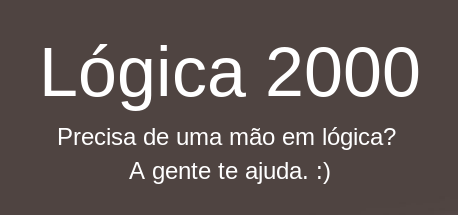
\includegraphics[scale=.6]{print1.png}
					\caption{Texto de abertura do site.}
				\end{figure}

			O projeto foi desenvolvido usando HTML5, CSS3, BootStrap e JavaScript. Os arquivos encontram-se hospedados em um repositório\footnote{https://github.com/mejnour/logica-2000} no GitHub.\\

				\begin{figure}[!h]
					\centering
					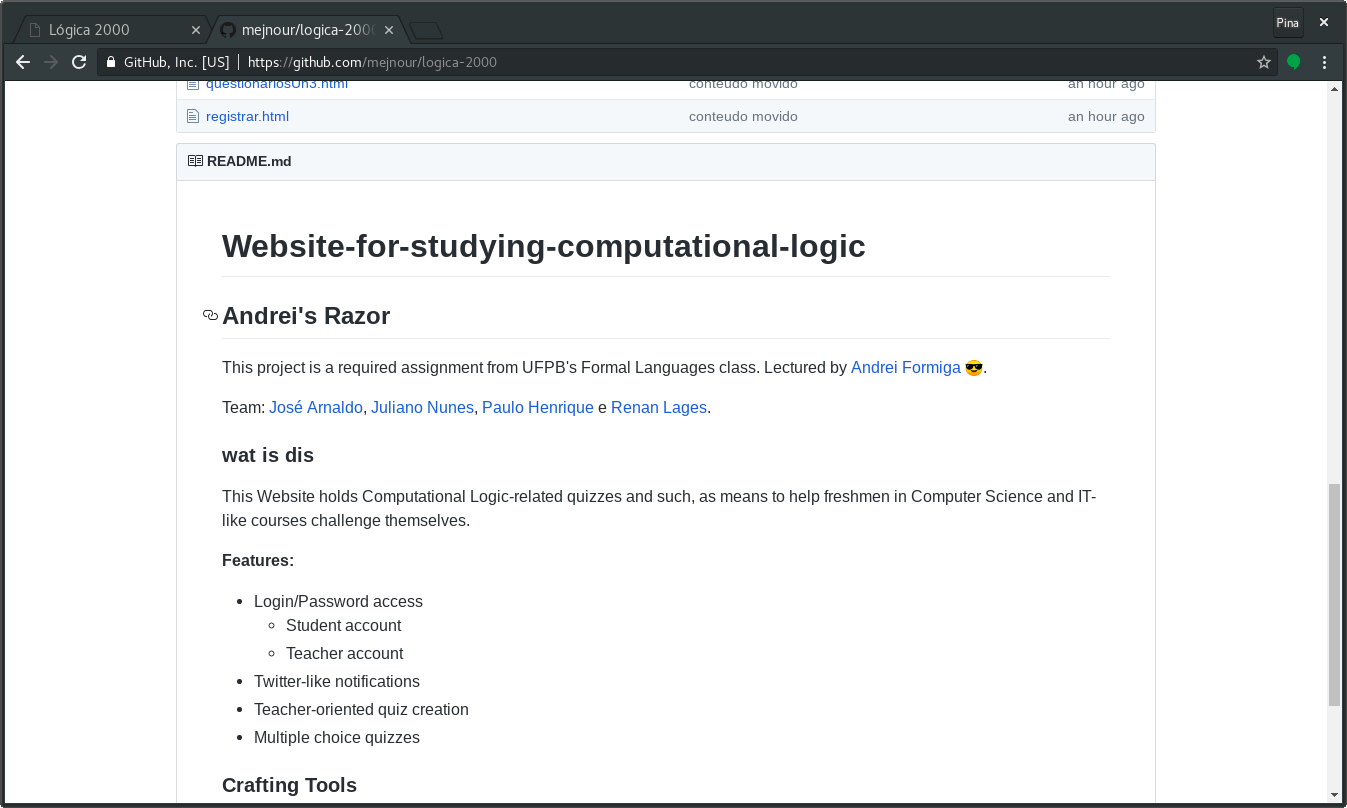
\includegraphics[scale=.2]{print1-1.png}
					\caption{README.md - Apresentação do Projeto no GitHub.}
				\end{figure}

			Como ambiente de desenvolvimento, usou-se os editores de texto Atom e Sublime Text.

			\pagebreak

		\subsection{Detalhes do Projeto}

			O projeto conta com as seguintes funcionalidades:

			\begin{itemize}
				\item Acesso usando Login/Senha;
				\item Conta de Estudante;
				\item Conta de Professor;
				\item Notificações direto do Professor;
				\item Criação de questionários no lado do Professor;
				\item Questionários de múltipla-escolha.
			\end{itemize}

			Na \emph{landing page}, o usuário depara-se com um texto de boas-vindas, botões de \emph{login} e registrar-se, além de atalhos em uma barra estática superior.

				\begin{figure}[!h]
					\centering
					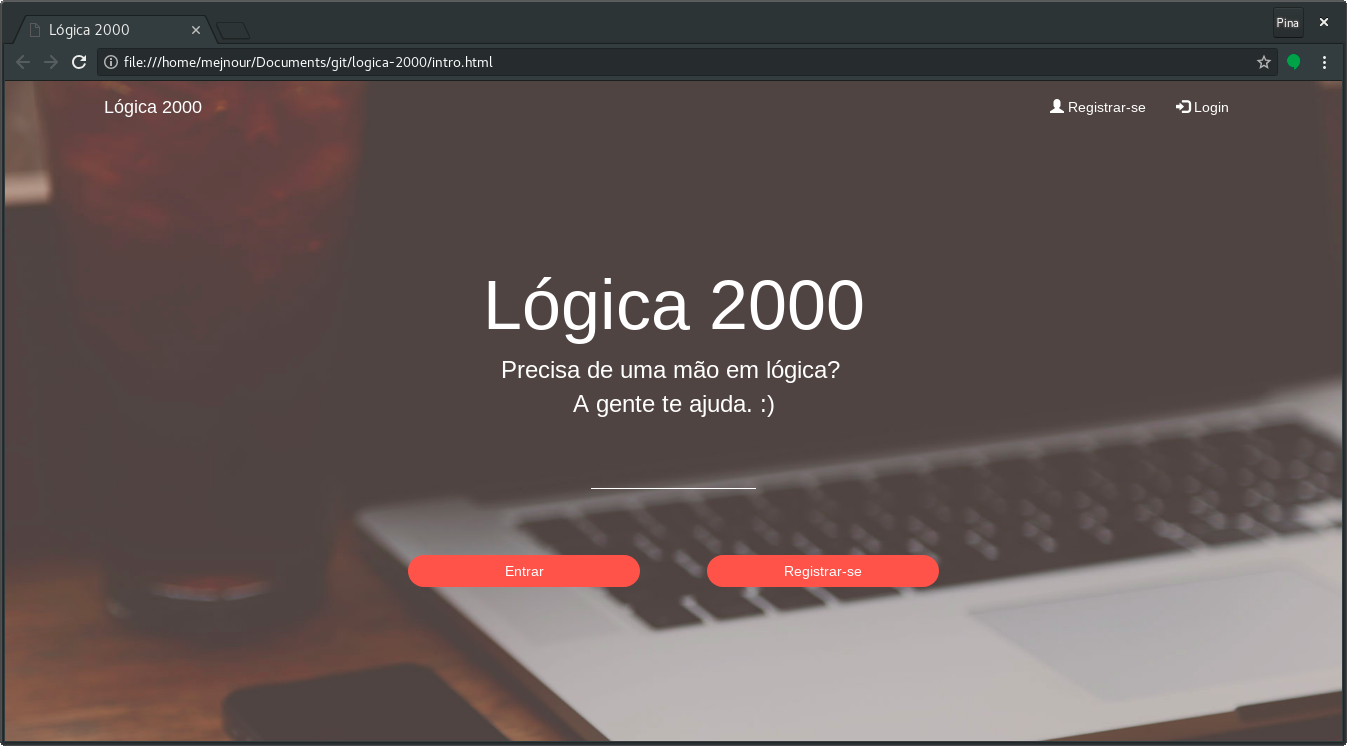
\includegraphics[scale=.3]{print2.png}
					\caption{\emph{Home} estática do site.}
				\end{figure}

				\pagebreak

			Ao clicar em \emph{Registrar-se}, o usuário é levado à tela de formulário, que exige e-mail válido e senha com, no mínimo, 6 caracteres, segue:

				\begin{figure}[!h]
					\centering
					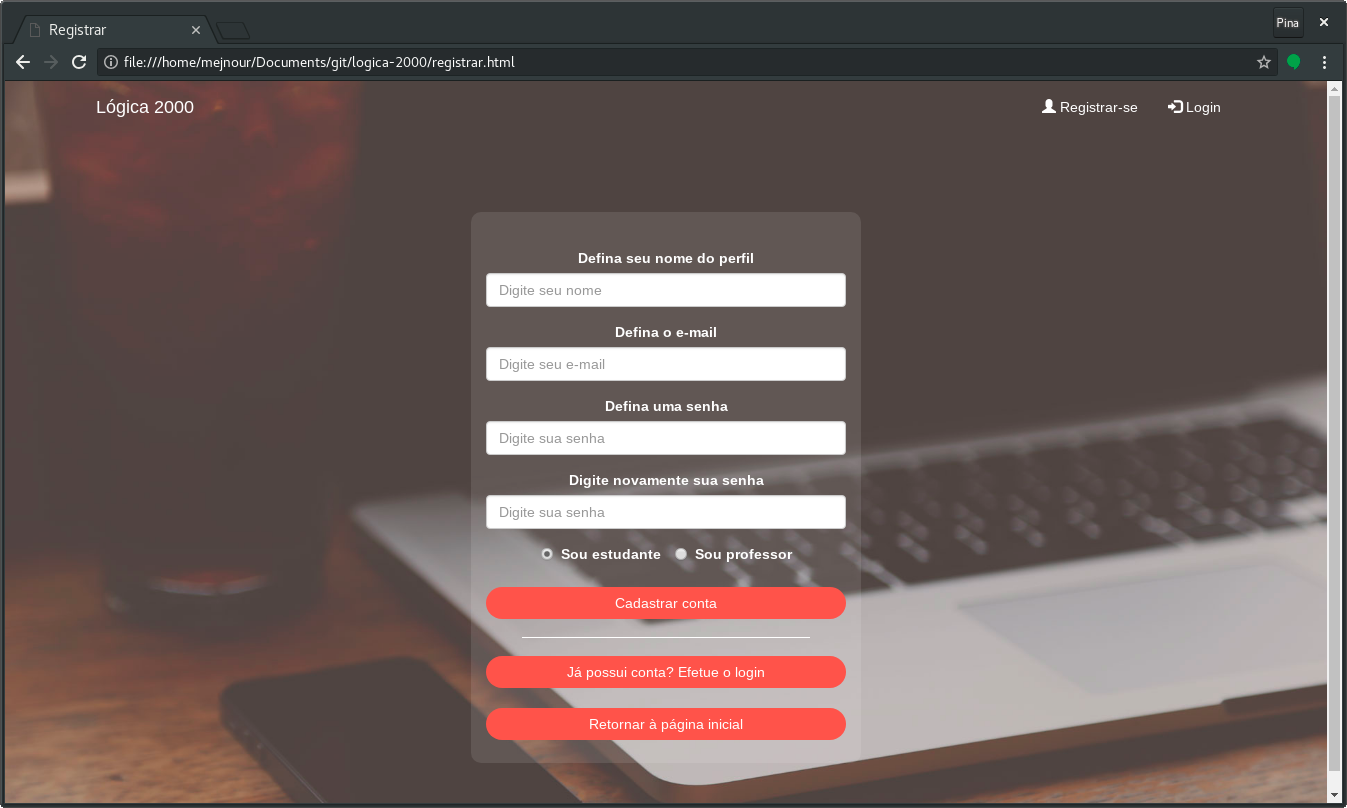
\includegraphics[scale=.32]{print3.png}
					\caption{Formulário de Registro.}
				\end{figure}

			Quando o usuário termina seu registro, o navegador o notifica do registro realizado com sucesso e o redireciona à página de \emph{Login}:

				\begin{figure}[!h]
					\centering
					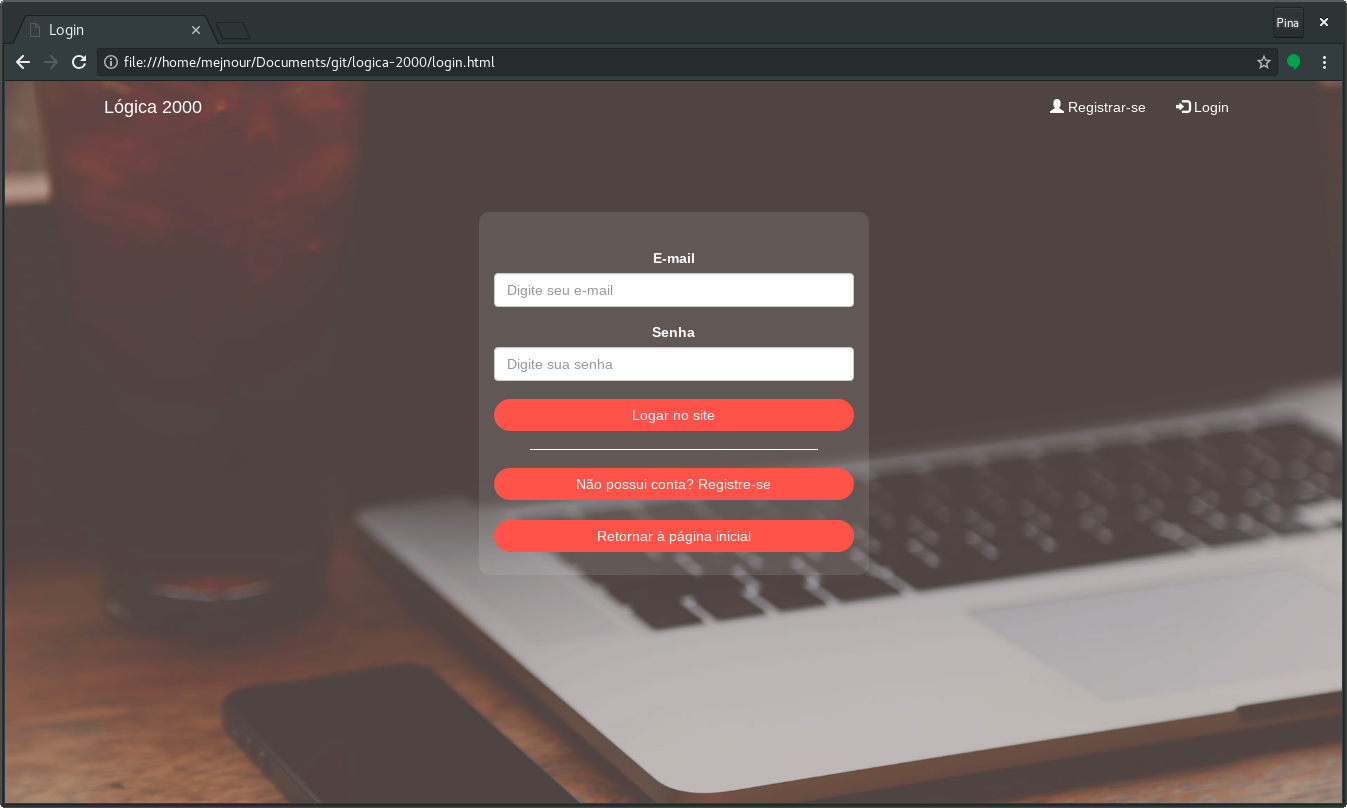
\includegraphics[scale=.32]{print4.png}
					\caption{\emph{Login screen}.}
				\end{figure}

				\pagebreak

			Quando o usuário entra os dados corretamente, o navegador o notifica que logou com sucesso:

				\begin{figure}[!h]
					\centering
					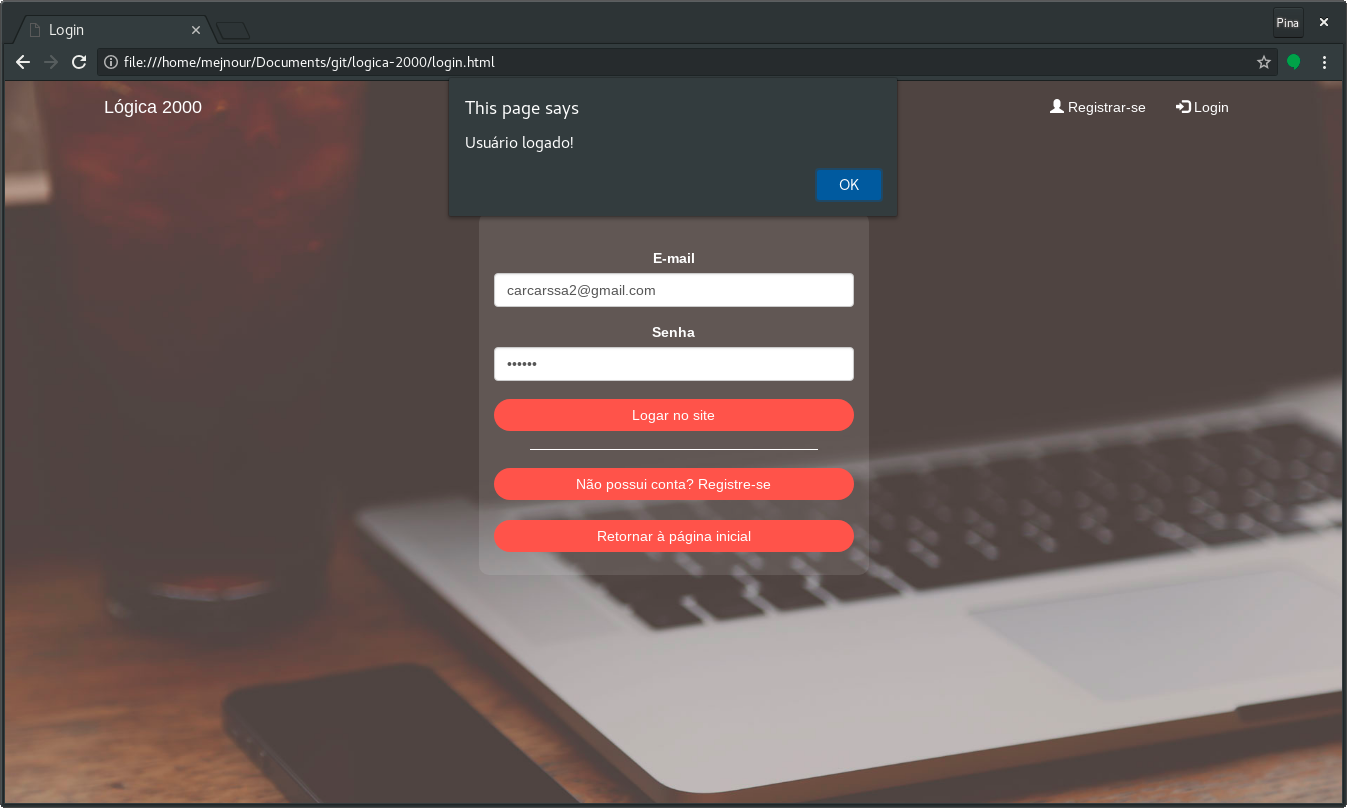
\includegraphics[scale=.32]{print5.png}
					\caption{Usuário logado com sucesso.}
				\end{figure}

			Já em uso da ferramenta, ele é recebido com uma mensagem de boas-vindas e as últimas notícias cadastradas pelo professor:

				\begin{figure}[!h]
					\centering
					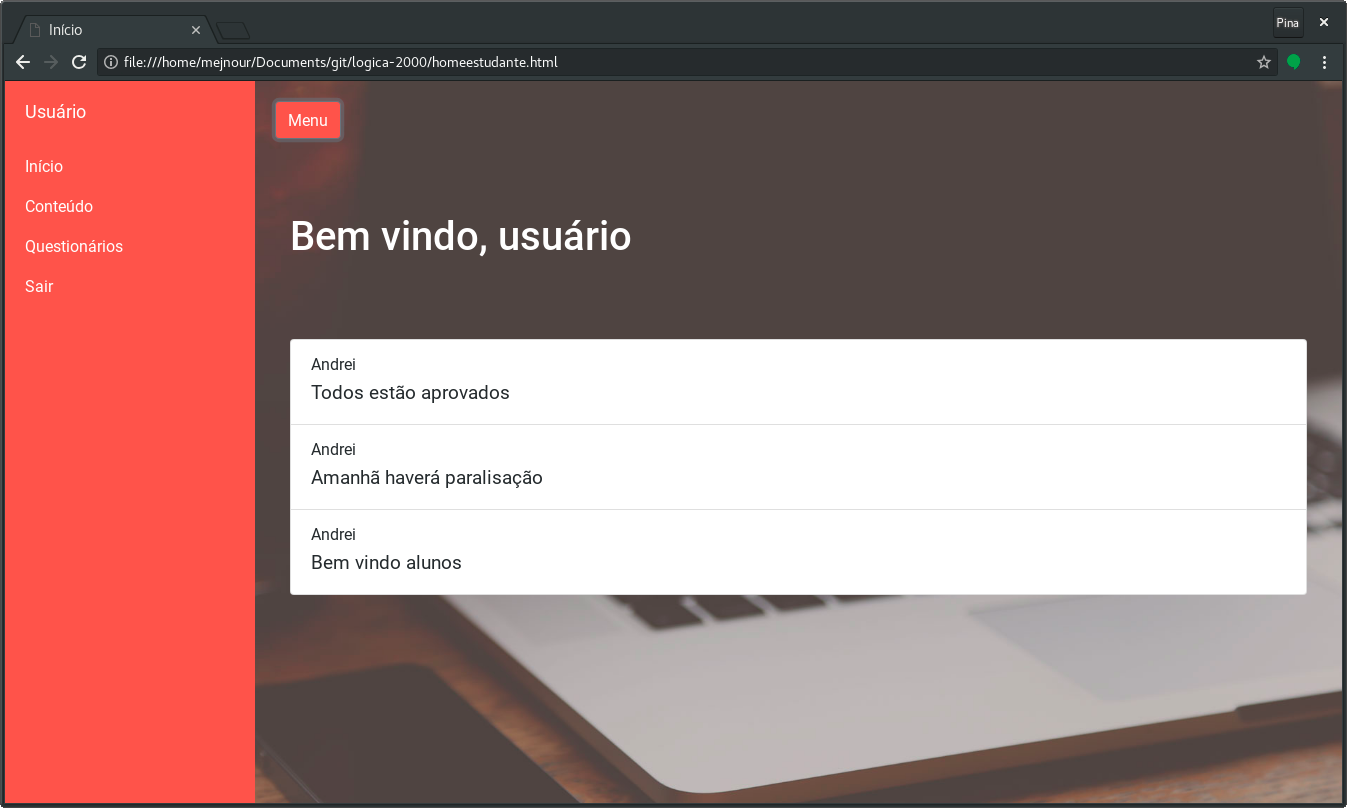
\includegraphics[scale=.32]{print6.png}
					\caption{Tela de Boas-vindas à ferramenta.}
				\end{figure}

			O menu é retrátil e dá acesso à página \textbf{Conteúdo}, onde ficariam textos e materiais de apoio adicionados tanto pelo professor quanto pela equipe de desenvolvimento:

				\begin{figure}[!h]
					\centering
					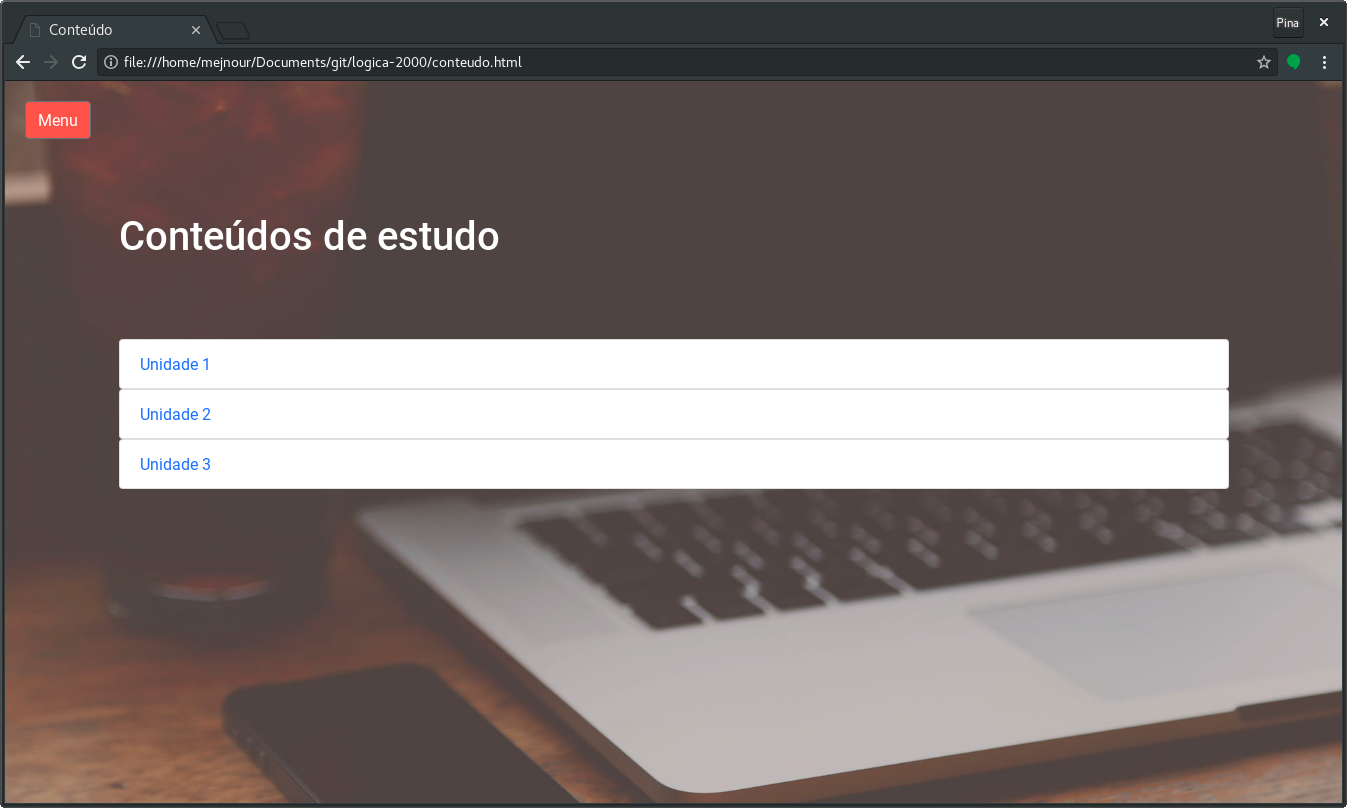
\includegraphics[scale=.32]{print7.png}
					\caption{Lista de Unidades em que se dividem os conteúdos cadastrados.}
				\end{figure}

			Acionando-se o menu retrátil novamente e selecionando-se a opção \emph{questionários}, o usuário é levado a uma lista de Unidades sob as quais está organizada uma série de questionários passíveis de cadastro pelo professor:

				\begin{figure}[!h]
					\centering
					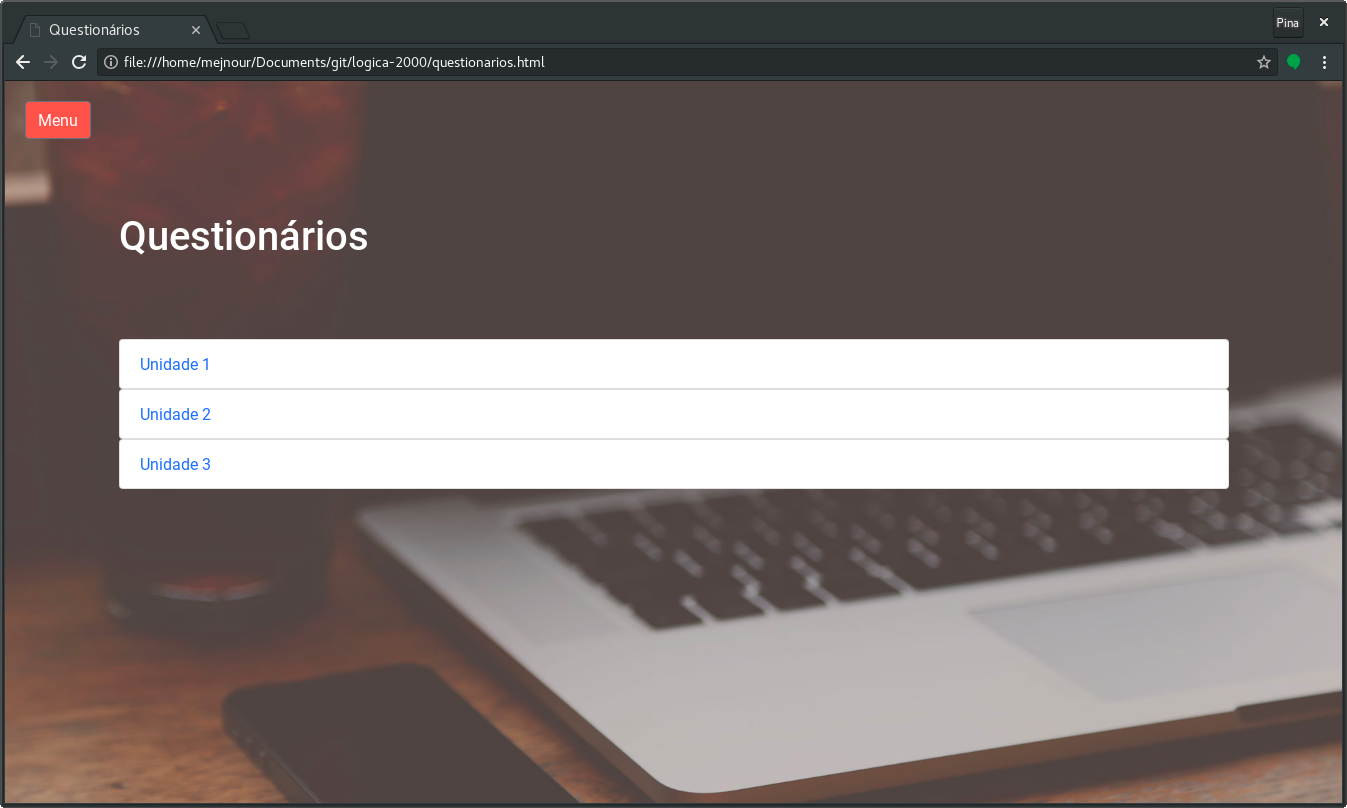
\includegraphics[scale=.32]{print8.png}
					\caption{Lista de Unidades em que se dividem os questionários cadastrados.}
				\end{figure}

			Dando acesso aos referidos questionários:

				\begin{figure}[!h]
					\centering
					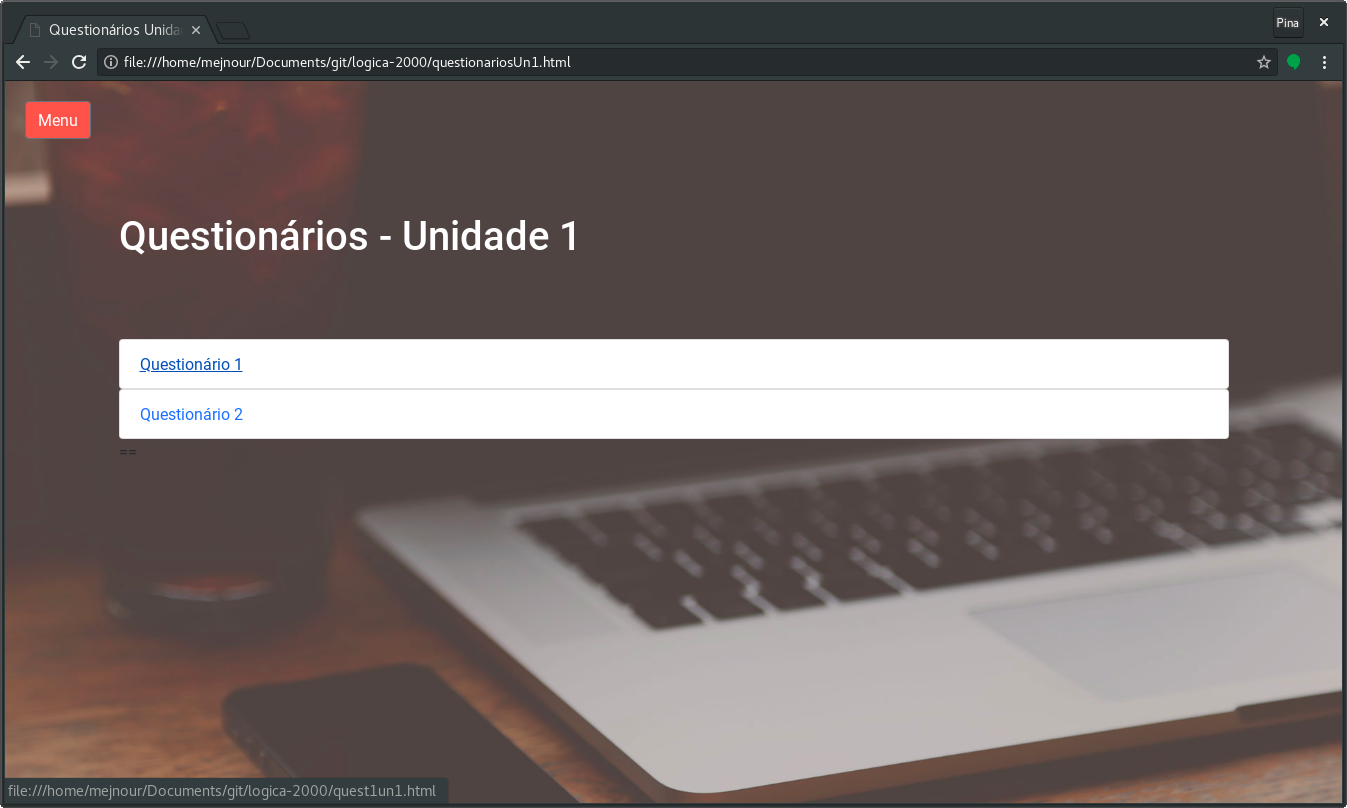
\includegraphics[scale=.32]{print9.png}
					\caption{Lista de questionários sob a Unidade selecionada.}
				\end{figure}

			E a um questionário específico de várias perguntas de múltipla escolha:

				\begin{figure}[!h]
					\centering
					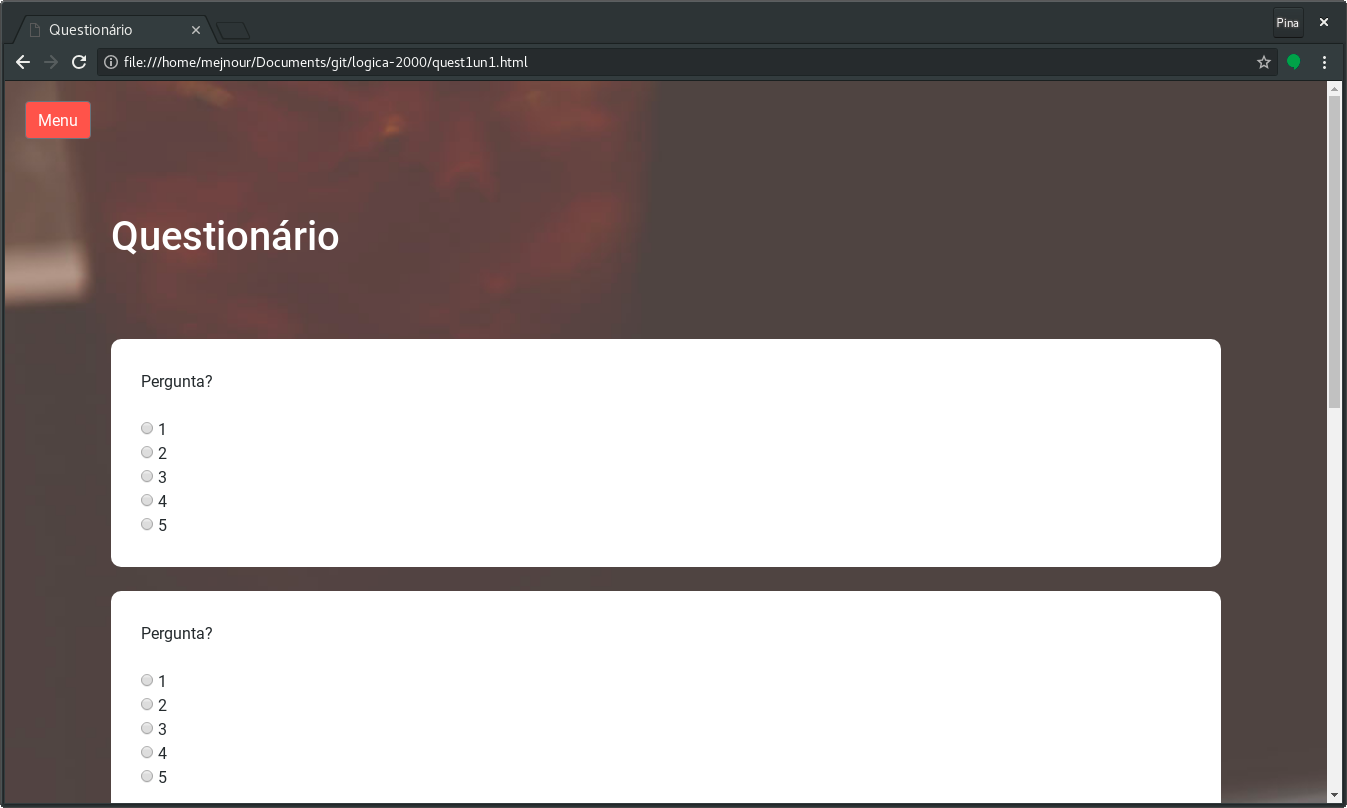
\includegraphics[scale=.32]{print10.png}
					\caption{Lista de questões de múltipla escolha.}
				\end{figure}

		\subsection{Dificuldades Encontradas}

			Este projeto de desenvolvimento web foi a primeira experiência de todos os integrantes do grupo, constituíndo, por si só, o desafio pessoal de aprender os conceitos básicos para se conseguir atingir os objetivos propostos.\\

			Em relação ao cronograma apresentado no pré-projeto, percebeu-se que o tempo delimitado para revisão bibliográfica foi curto, deixando algumas funcionalidades antes propostas, inacabadas e, por isso, retiradas da apresentação final e deste relatório. São elas:

			\begin{itemize}
				\item Integração dos Usuários em Rede Social; e
				\item Ranking dos Usuários por questões respondidas.
			\end{itemize}

			A saber, é interesse dos membros continuar a desenvolver as referidas funcionalidades durante o período de recesso entre os períodos 2017.2 e 2018.1.

		\subsection{Possíveis Melhorias}

			Durante o desenvolvimento, foram feitas escolhas onde se prezou pelo rápido desenvolvimento em detrimento da vontade geral do grupo de desenvolver todos os aspectos pensados pela equipe. O site pode melhorar em vários aspectos estéticos e organizacionais bem como em outros pontos que são listados a seguir.

			\begin{itemize}
				\item \textbf{Analisador em Tempo Real:} A ideia é conseguir que, enquanto o usuário estiver respondendo determinada questão do site, sua resposta seja interpretada em tempo real e sugestões apareçam, tal como acontece em teclados mobile -- com a diferença de que, a invés de palavras sugeridas, as sugestões fossem passagens de texto contidas no banco do dades, podendo o usuário se beneficiar caso esteja caindo em um erro comum previamente identificado.

				\item \textbf{Página Sobre:} Poder-se-ia, explanando melhor as diretrizes do projeto, hangariar colaboradores para melhorar o banco de dados, disponibilizando ao professor, não somente uma ferramenta de criação de questões, como algum acervo criado pela comunidade.
			\end{itemize}

	\section{Conclusão}

		Durante o período 2017.2 da UFPB, na disciplina de Linguagens Formais e Autômatos, ministrada pelo Professor Andrei Formiga, foi possível aos alunos terem um primeiro contato com o que há de ponta no desenvolvimento científico relativo à Computação.\\

		Desde uma revisão dos conteúdos baselares, passando por complexidade de algoritmos, entre outros tópicos, ficou claro aos atendentes da disciplina que o universo da computação era muito mais amplo e profundo do que descreviam os pequenos mapas simbólicos da situação dados pelos professores até então.\\

		Assim, a possibilidade de desenvolver um projeto aberto, sem finalidade previamente definida pelo professor, foi uma oportunidade única de explorar ferramentas não usuais nas tradicionais disciplinas do curso, contribuíndo com a experiência que é sanar uma curiosidade e o treinamento profissional auto-imposto.


\end{document}
